% 2009 年重庆卷文科第 18 题：五面体 ABCDEF（AB∥DC，FA⊥平面 ABCD，ABFE 为平行四边形）。
% 来源 PDF：普通高考/2009/2009重庆文.pdf，SHA-256 c4d433586be8144d34c8ee2d4074c6308f53ffe84aa3a8a7ea28bb6f0cf86a39。
% 原页：第 1 页（A3 三栏）第 3 栏下部，书页码 505。
% 重绘依据：由题设取 A(0,0,0)、B(-√2,0,0)、D(0,2,0)、C(-2,2,0)、F(0,0,1)、E(√2,0,1)。
%   可见外轮廓 F-E-D-C-B-F 为实线；FA、AB、AD 为被遮挡或内部辅助线，画虚线。
%   投影取 (x,y,z) -> (x+0.35y, 2.20z+0.28y)。
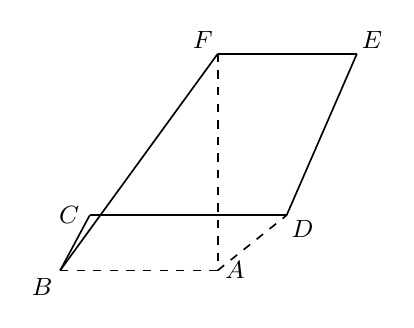
\begin{tikzpicture}[semithick, scale=1.25, every node/.style={inner sep=1.5pt, font=\small}]
  \coordinate (A) at (0.000,0.000);
  \coordinate (B) at (-1.600,0.000);
  \coordinate (C) at (-1.300,0.560);
  \coordinate (D) at (0.700,0.560);
  \coordinate (F) at (0.000,2.200);
  \coordinate (E) at (1.414,2.200);

  % 外轮廓
  \draw (F) -- (E);
  \draw (E) -- (D);
  \draw (D) -- (C);
  \draw (C) -- (B);
  \draw (B) -- (F);

  % 内部与遮挡线
  \draw[dashed] (F) -- (A);
  \draw[dashed] (A) -- (B);
  \draw[dashed] (A) -- (D);

  % 标注
  \node[right=1pt] at (A) {$A$};
  \node[below left=1pt] at (B) {$B$};
  \node[left=2pt] at (C) {$C$};
  \node[below right] at (D) {$D$};
  \node[above left] at (F) {$F$};
  \node[above right] at (E) {$E$};
\end{tikzpicture}
